\documentclass[11pt]{article}
% =====================================================================
%  CTX-pro family --- the program-feature category, explained.
%  Standalone explainer matched to what the arbiter rule actually
%  measures (depth_reach), plus the honest refuted/inconclusive faces.
%  Compile: pdflatex ctx_pro_categories.tex   (needs tikz + pgfplots + listings)
% =====================================================================
\usepackage[margin=1in]{geometry}
\usepackage{amsmath,amssymb}
\usepackage{xcolor}
\usepackage{listings}
\usepackage{booktabs}
\usepackage{tikz}
\usepackage{pgfplots}
\pgfplotsset{compat=1.16}
\usetikzlibrary{arrows.meta,positioning,shapes.geometric}

\definecolor{winc}{RGB}{30,120,60}   % winner (ctx helps) green
\definecolor{losc}{RGB}{190,60,60}   % loser  (no ctx)    red
\definecolor{codebg}{RGB}{246,246,248}
\definecolor{kw}{RGB}{40,60,150}
\definecolor{cmt}{RGB}{120,120,120}
\definecolor{str}{RGB}{160,60,20}

\lstdefinestyle{c}{
  language=C, basicstyle=\ttfamily\small, backgroundcolor=\color{codebg},
  keywordstyle=\color{kw}\bfseries, commentstyle=\color{cmt}\itshape,
  stringstyle=\color{str}, numbers=none, frame=single, framerule=0pt,
  framesep=6pt, breaklines=true, showstringspaces=false, xleftmargin=4pt,
}

% A small "metric & rule" box used under every category.
\newcommand{\metricbox}[4]{%
  % #1 tool  #2 metric (plain meaning)  #3 verify rule  #4 real example
  \par\smallskip\noindent\fbox{\parbox{\dimexpr\linewidth-2\fboxsep-2\fboxrule}{%
  \footnotesize
  \textbf{Tool:}~\texttt{#1}\\[2pt]
  \textbf{Metric:}~#2\\[2pt]
  \textbf{Verify rule (the arbiter fires this, no LLM):}~\texttt{#3}\\[2pt]
  \textbf{Real example:}~#4}}\par\smallskip}

\title{\textbf{The CTX-pro family: finer-grained coverage keeps the seed that goes deeper}}
\author{}
\date{}

\begin{document}
\maketitle
\vspace{-3em}

\paragraph{Backdrop.} \emph{CTX-pro} collects the roadblocks where a fuzzer with
\emph{context-sensitive coverage} (\texttt{naive\_ctx}) gets through while the
same byte-mutation fuzzer with a plain edge map (\texttt{naive}) stays stuck.
Both fuzzers mutate bytes the same blind way --- the \emph{only} difference is
what counts as ``new coverage.'' Plain \texttt{naive} has one slot per control
edge: the first input to cross edge $E$ marks it done, and any later seed that
crosses $E$ again --- from a deeper loop iteration, a deeper recursion level, or a
\emph{different caller chain} --- earns no credit and is thrown away.
\texttt{naive\_ctx}'s \texttt{CtxHook} folds the \emph{caller chain} into the
map index, so each \emph{(call-context, edge)} pair is its own slot. Re-entering
the same edge one loop deeper, or reaching the same function through a new
caller, now registers as fresh coverage --- so the seed is \emph{kept}. That
retention manufactures a \emph{depth gradient}: the corpus accumulates partial,
mid-progress seeds, and a rare deep continuation becomes reachable from a
retained mid-parse seed instead of having to appear all at once. Unlike I2S/VP
there is no ``key beside the lock'' here --- there is no value to paste; the
advantage is purely \emph{which seeds survive}. Counts are validated
roadblocks~($n$). Of the 53 CTX-pro memberships, \textbf{14 validate} as the one
discriminable mechanism below; the remaining 39 are honestly \emph{inconclusive}
(see ``The other two faces'').

% =====================================================================
\section*{1.\ \ Iteration / path-depth reach \hfill {\normalsize\texttt{ctx\_iteration\_path\_depth} ($n=14$)}}
The blocker sits one step \emph{deeper} along a path the loser corpus never
retains seeds for: an extra loop iteration, a deeper recursion level, the same
function reached through a new call context. \texttt{naive}'s saturated edge map
discards the mid-progress seeds that would get there; \texttt{naive\_ctx}'s
context-split map keeps them, so its corpus drives the blocker line to a strictly
higher per-seed execution count (or actually takes the blocked side). This is
the \emph{only} face of the ctx advantage that shows up per-seed, and the only
CTX-pro mechanism real campaign data can discriminate.

\begin{lstlisting}[style=c]
// libxml2  parser.c : xmlParseCharRef()  -- decimal char reference  &#dddd...;
// the digit-scan loop; the gate is one extra iteration past a depth threshold
while (RAW != ';') {                      // RAW walks the &#... digits
    val = val * 10 + (CUR - '0');
    if (count++ > 20) {                   // <-- blocker (libxml2/6467, L2353):
        xmlFatalErr(...); return 0;       //     only seeds with >20 digits reach it
    }
    NEXTL(...);
}
\end{lstlisting}

\noindent\textbf{How we know it is really the depth mechanism.} If the winner
corpus is winning by reaching the line \emph{deeper}, then running each arm's
saved seeds through the instrumented binary should show the \texttt{naive\_ctx}
seeds executing the blocker line far more times per seed (and taking the blocked
side) than \texttt{naive}'s. We run the seeds and read the line's execution count
straight from the \texttt{llvm-cov} dump; the rule asks for at least a
$2\times$ per-seed lift \emph{and} that the winner is the deeper one.

\metricbox{depth\_reach}
{\texttt{depth\_lift} $=\dfrac{\text{winner per-seed blocker-line execs}}{\max(\text{loser per-seed blocker-line execs},\,1)}$; \ \texttt{winner\_deeper} = winner reaches the line strictly deeper}
{depth\_lift >= 2.0 AND winner\_deeper == True}
{libxml2/6467 (\texttt{xmlParseCharRef}, \texttt{count++>20}) --- the
\texttt{naive\_ctx} corpus runs the gate line $89.7$ times per seed vs
\texttt{naive}'s $12.4$, so \texttt{depth\_lift}$=7.26$ and the blocked side is
taken $7.0\times$ more (\texttt{side\_lift}$=7.02$): only the context-retained
corpus carries the $>$20-digit references that trip the loop past threshold.}

\begin{center}
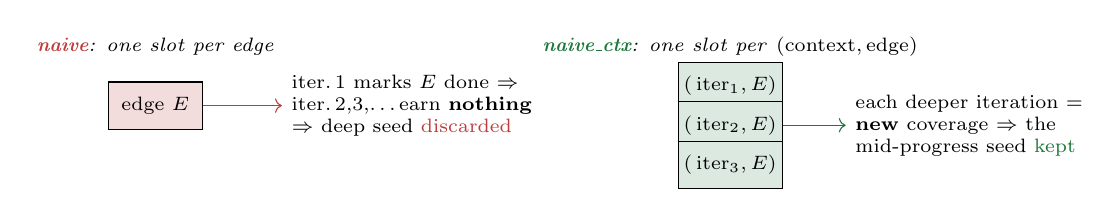
\begin{tikzpicture}[font=\footnotesize,
  slot/.style={draw,minimum height=6mm,minimum width=12mm,font=\scriptsize,inner sep=2pt},
  full/.style={slot,fill=losc!18},
  ctxslot/.style={slot,fill=winc!16},
  lbl/.style={font=\scriptsize\itshape}]
% ---- LEFT: naive bare edge map (one slot per edge, saturates) ----
\node[lbl] (nlab) at (0,1.05) {\textcolor{losc}{\textbf{naive}}: one slot per edge};
\node[full] (e1) at (0,0.3) {edge $E$};
\node[right=10mm of e1,align=left,font=\scriptsize] (nsat)
  {iter.\,1 marks $E$ done $\Rightarrow$\\ iter.\,2,3,\dots earn \textbf{nothing}\\
   $\Rightarrow$ deep seed \textcolor{losc}{discarded}};
\draw[->,losc] (e1.east) -- (nsat.west);
% ---- RIGHT: naive_ctx context-split map ----
\begin{scope}[xshift=7.3cm]
\node[lbl] (clab) at (0,1.05) {\textcolor{winc}{\textbf{naive\_ctx}}: one slot per \emph{(context,\,edge)}};
\node[ctxslot] (c1) at (0,0.55) {$(\,\text{iter}_1,E)$};
\node[ctxslot] (c2) at (0,0.05) {$(\,\text{iter}_2,E)$};
\node[ctxslot] (c3) at (0,-0.45){$(\,\text{iter}_3,E)$};
\node[right=8mm of c2,align=left,font=\scriptsize] (cret)
  {each deeper iteration =\\ \textbf{new} coverage $\Rightarrow$ the\\
   mid-progress seed \textcolor{winc}{kept}};
\draw[->,winc] (c2.east) -- (cret.west);
\end{scope}
\end{tikzpicture}\\[4pt]
% ---- per-seed depth bar comparison for the real example ----
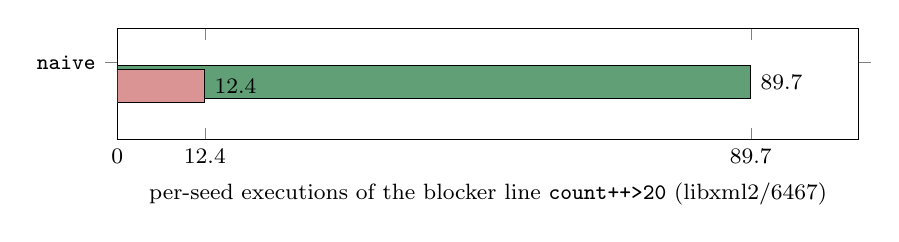
\begin{tikzpicture}
\begin{axis}[
  width=11cm, height=3.0cm, xbar, xmin=0, xmax=105,
  bar width=12pt, enlarge y limits=0.8,
  symbolic y coords={naive, naivectx},
  ytick=data, yticklabels={\texttt{naive}, \texttt{naive\_ctx}},
  xtick={0,12.4,89.7}, xticklabel style={font=\footnotesize},
  yticklabel style={font=\footnotesize},
  nodes near coords, every node near coord/.append style={font=\footnotesize},
  xlabel={\footnotesize per-seed executions of the blocker line \texttt{count++>20} (libxml2/6467)},
]
\addplot[fill=winc!70] coordinates {(89.7,naivectx)};
\addplot[fill=losc!55] coordinates {(12.4,naive)};
\end{axis}
\end{tikzpicture}\\[-1pt]
{\footnotesize Same blind byte mutation on both arms; the context-split map keeps
the seeds that re-enter the digit loop, so \texttt{naive\_ctx} drives the gate
line $7.26\times$ deeper (\texttt{depth\_lift}) and trips the $>$20-iteration
side the loser never assembles.}
\end{center}

\paragraph{What the rule rules \emph{out}.} A value/byte-solving roadblock
mis-bucketed into this \texttt{naive\_ctx}$>$\texttt{naive} shape would reach the
blocker line at the \emph{same} depth and differ only in operand bytes ---
\texttt{depth\_lift}$\approx 1$, rule fails. A branch where \texttt{naive} is
actually the deeper arm (e.g.\ harfbuzz/5237, \texttt{depth\_lift}$=0.14$) fails
on \texttt{winner\_deeper}. So the rule is both falsifiable and discriminating:
it fires only when the winner's edge is genuinely the deeper-reaching corpus.

% =====================================================================
\section*{The other two faces (why only 14 of 53 validate)}
CTX-pro is a \emph{non-local} feedback mechanism, and most of its surface does
not leave a per-seed fingerprint. We tested two further faces honestly; neither
rescued the residual, and we leave them on the record rather than force a label.

\paragraph{Face 2 --- corpus-scale inflation (\emph{refuted on the measured arms}).}
The textbook story for context-sensitive coverage is that it admits \emph{many
more} seeds --- the same edge through a new caller chain counts as new coverage
--- so \texttt{naive\_ctx} should hoard a strictly larger, more context-diverse
saved corpus than \texttt{naive}, whether or not any single seed reaches the
blocker deeper. That is a corpus-\emph{scale} signature \texttt{depth\_reach} is
blind to, so we built a separate arm-level test.

\metricbox{corpus\_size\_ratio}
{\texttt{corpus\_count\_ratio} $=\dfrac{\text{median \# saved seeds, naive\_ctx}}{\text{median \# saved seeds, naive}}$ across trials \ ($>1$ = ctx hoards more)}
{corpus\_count\_ratio >= 1.5}
{Measured on this shape's targets: \texttt{harfbuzz} $=0.924$, \texttt{sqlite3}
$=0.956$ (composition-entropy ratios $\approx 1.01$) --- both \emph{below} $1.0$,
so the corpus-inflation mechanism is \textbf{refuted} on the measured arms. The
rule is kept as a genuine falsifiable test (it \emph{can} fire $\ge 1.5$ on a
target where ctx truly inflates), but here it correctly does not fire.}

\paragraph{Face 3 --- the value route is structurally unavailable
(\emph{decidable:\,false}).} The 39 remaining branches fail both kept rules:
their per-seed depth does not separate ($\texttt{depth\_lift}<2.0$) and their arm
does not hoard a bigger corpus ($\texttt{corpus\_count\_ratio}<1.5$). Several
\emph{do} carry a literal operand (libpng \texttt{color\_type==3}; libxml2
overlong-encoding; harfbuzz codepoint switch arms), which is why a byte/value
tool looks tempting --- but the resolving arm is \texttt{naive\_ctx}, which has
\emph{neither} \texttt{value\_profile} \emph{nor} \texttt{cmplog}. There is no
I2S operand-substitution contrast for \texttt{operand\_enrichment} to read and no
Hamming gradient for \texttt{value\_distance\_reached} to climb; the cards say
plainly the bytes are \emph{not} the blocker (``no extra byte requirement beyond
naive's'') --- retention/scheduling is. Applying a value tool here would
manufacture a comparison the mechanism cannot produce (a G2 violation: the
winning arm has no value-solver). This is a \emph{mechanism-level} rejection
valid for every residual branch on both servers, so the subgroup converges
honestly to \texttt{decidable:\,false} rather than to a forced label.

% =====================================================================
\section*{At a glance}
\begin{center}\small
\begin{tabular}{@{}p{3.8cm}clp{5.2cm}@{}}
\toprule
\textbf{Face} & \textbf{$n$} & \textbf{Tool / metric} & \textbf{Outcome / one-line reason} \\
\midrule
iteration / path-depth reach & 14 & depth\_reach / \texttt{depth\_lift}, \texttt{winner\_deeper} & \textbf{validated}: context-split map keeps the seed that re-enters the loop / reaches the line deeper \\
corpus-scale inflation        & 0  & corpus\_size\_ratio / \texttt{corpus\_count\_ratio} & \emph{refuted} on measured arms ($0.92$, $0.96 < 1.5$); kept as a falsifiable test \\
value route (literal operand) & 0  & operand\_enrichment / value\_distance\_reached & \texttt{decidable:false}: naive\_ctx has no I2S/VP arm to read (G2) \\
\midrule
\textbf{CTX-pro validated}    & \textbf{14} & & (of 53 memberships; 39 honestly inconclusive) \\
\bottomrule
\end{tabular}
\end{center}

\noindent\footnotesize Counts and example metrics regenerated from
\texttt{bench/dataset.jsonl} / \texttt{bench/roadblock\_facts.csv}; verify rules
are the deterministic arbiter rules (no LLM in the decision). The refuted and
\texttt{decidable:false} faces are reported deliberately --- an honest
\texttt{inconclusive} is the correct outcome for a non-local mechanism with no
cheap discriminating signal, not a gap to paper over.
\end{document}
